% Author: Seongjin Lee 
% Gyeongsang National University, Korea 
% 
% 2017-03-06
%

\documentclass[newPxFont,sthlmFooter,nooffset]{beamer}
\usepackage{kotex}
%\usetheme{sthlm}
\usepackage{../style/beamerthemesthlm}
\hypersetup{pdfauthor={Seongjin Lee (insight@gnu.ac.kr)},
            pdfsubject={Data Structure and Algorithm, Lecture Note},
            pdfkeywords={Data Structure, Algorithm, Lecture, Note},
            pdfmoddate={D: \pdfdate},
            pdfcreator={Seongjin Lee}}

%\setbeamertemplate{footline}[text line]{%
%    \parbox{\linewidth}{\vspace*{-8pt} \insertsectionhead  \hfill\insertshortauthor\hfill\insertpagenumber}}
%\setbeamertemplate{navigation symbols}{}


\setbeamertemplate{blocks}[rounded]

\title{Data Structure and Algorithm}
\subtitle{Class 4}
\author[SJL]{Seongjin Lee}
\institute{\href{mailto:insight@gnu.ac.kr}{insight@gnu.ac.kr}\\\url{http://resourceful.github.io}\\Systems Research Lab.\\GNU}
\date{2017-03-06} 

\begin{document}



\frame[plain,t]{\titlepage} 

\frame{\frametitle{Table of contents}\tableofcontents} 


%---------------------------------------------------------
\section{Makefile} 
\begin{frame}[t]
  \frametitle{Make}

  \begin{itemize}
  \item Stuart Feldman developed make in April in 1976 at Bell Labs

  \item Received 2003 ACM Software system Award for the tool

  \item It is utility that automatically builds executable programs 
and libraries from source code by reading file called makefile

  \end{itemize}
  \begin{center}
    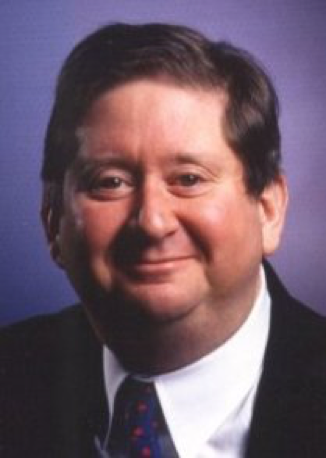
\includegraphics[width=0.3\textwidth]{figures/fig01_feldman.png}
  \end{center}

\end{frame}


\begin{frame}[t, fragile]
  \frametitle{Problem of multiple source files and repetitive
    routines}
  
Used to detect a change made to an image file and the transformation action might be converted the file to some specific format
\begin{itemize}
\item {\small Also can be used to copy the result into a content management
  system, and then send e-mail to a predefined set of users to note
  the changes}
\end{itemize}

\begin{columns}
\begin{column}{0.3\textwidth}
\begin{codedefnb}
/* main.c */
#include "foo.h''
...      
\end{codedefnb}
\end{column}
\begin{column}{0.3\textwidth}
\begin{codedefnb}
/* sub.c*/
#include “foo.h”
#include “bar.h”
…      
\end{codedefnb}
\end{column}
\begin{column}{0.3\textwidth}
\begin{codedefnb}
/* utmost.c*/
#include “bar.h”
#include “baz.h”
…     
\end{codedefnb}
\end{column}
\end{columns}
\begin{itemize}
\item If foo.h is changed – main.c and sub.c must be recompiled

\item If foo.h is changed but forgot to compile sub.c, the program might not work correctly

\end{itemize}





It can be used not only for compiling programs, but also for to produce output files from several input files such as TeX

Comment starts with \# and continues to the end  of the line




\end{frame}

\begin{frame}[t]
  \frametitle{Syntax of Makefile}

Makefile consists of a set of dependencies and rules
\begin{itemize}
\item A dependency has a target (a file to be created) and set of
  source files upon which it is dependent
\item The rules describe how to
  create the target from the dependent files
\end{itemize}

Typically target is a single executable file
\end{frame}

\begin{frame}[t]
  \frametitle{Make}

  \begin{center}
    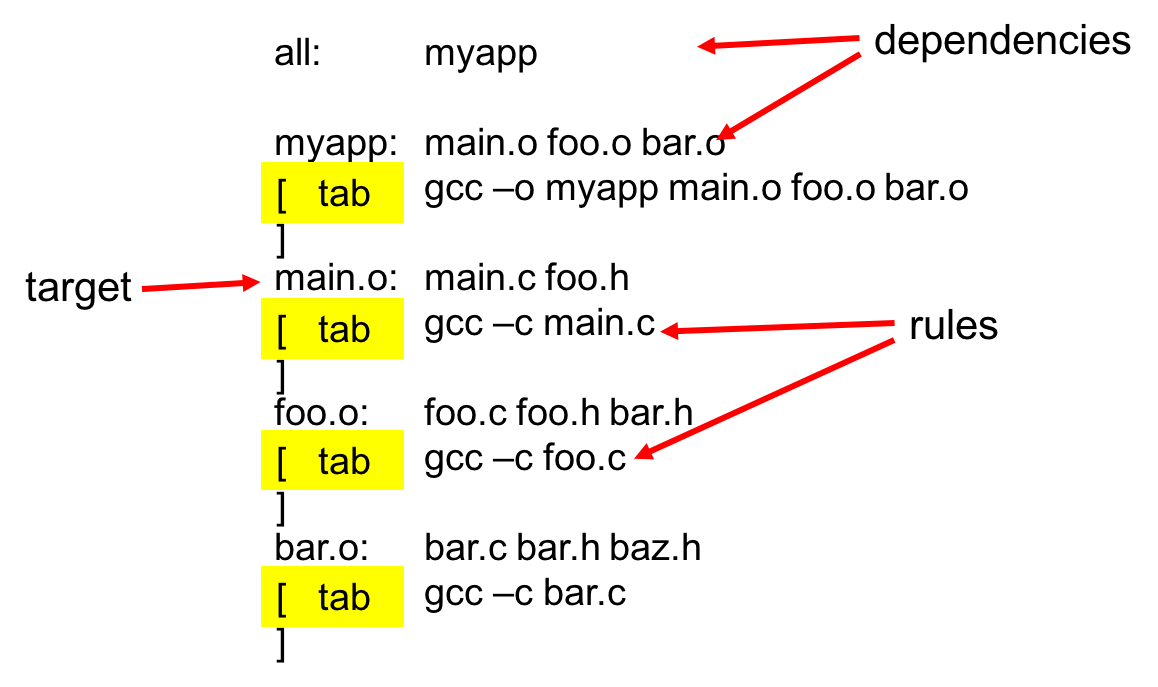
\includegraphics[width=0.9\textwidth]{figures/fig02_structure.png}
  \end{center}

\end{frame}

\begin{frame}[t, fragile]
  \frametitle{Syntax of Makefile}
\begin{columns}
\begin{column}{0.3\textwidth}
\lstinputlisting[lineskip=1pt, numbers=left]{codes/main.c}
\end{column}
\begin{column}{0.3\textwidth}
\lstinputlisting[lineskip=1pt, numbers=left]{codes/foo.c}
\end{column}
\begin{column}{0.3\textwidth}
\lstinputlisting[lineskip=1pt, numbers=left]{codes/bar.c}
\end{column}
\end{columns}

\begin{columns}
\begin{column}{0.4\textwidth}
\begin{codedefnb}
> make
> make
\end{codedefnb}
\end{column}
\begin{column}{0.4\textwidth}
\begin{codedefnb}
> touch bar.h
> make
> rm bar.o
> make
\end{codedefnb}
\end{column}
\end{columns}


\end{frame}



\begin{frame}[t]
  \frametitle{Macros in a Makefile}
Define a macro in a makefile by writing 
\begin{itemize}
\item \texttt{MACRONAME=value}
\end{itemize}


Accessing the value of MACRONAME by writing 
\begin{itemize}
\item \texttt{\$(MACRONAME) or \${MACRONAME}}
\end{itemize}


Usually macros are defined inside the makefile
\begin{itemize}
\item But can be specified by calling make with macro definition
\item \texttt{make CC=c89}
\end{itemize}


\end{frame}

\begin{frame}
  \frametitle{Makefile with macros}
  \begin{columns}
    \begin{column}{0.5\textwidth}
      \lstinputlisting[lineskip=1pt, numbers=left, linerange=1-14]{codes/Makefile1}
    \end{column}
    \begin{column}{0.45\textwidth}
      \lstinputlisting[lineskip=1pt, numbers=left, linerange=15-32]{codes/Makefile1}
    \end{column}
  \end{columns}

\end{frame}

\begin{frame}[t]
  \frametitle{Special Internal Macros}
  \begin{itemize}
  \item \texttt{\$?} - List of prerequisites (files the target depends
    on) changed more recently than the current target
  \item \texttt{\$@} - Name of the current target
  \item \texttt{\$<} - Name of the Current prerequisite
  \item \texttt{\$*} - Name of the current prerequisite, without any suffix
  \item \texttt{@} - (applies to rules) Tell make not to print the command to standard output before executing it
  \item \texttt{-} - (applies to rules) Tell make to ignore any errors

  \end{itemize}
\end{frame}

\begin{frame}[t]
  \frametitle{Multiple Targets}
\lstinputlisting[lineskip=1pt, numbers=left]{codes/Makefile2}  
\end{frame}

\end{document}
